\graphicspath{ {res/img/} }

\subsection{Accessibilità}
%TODO
%MEMO: per i problemi e le soluzioni addottate per l'accessibilita' vedere:
%https://github.com/Hexamini/PassioneKaraoke/issues?utf8=%E2%9C%93&q=is%3Aissue+milestone%3AAccessibilit%C3%A0+
Il sito è stato sviluppato utilizzando solamente codice HTML5. Per i fogli di stile si è invece deciso di applicare CSS 3.0, per poter sfruttare nuove tecnologie grafiche e ridurre al minimo l'utilizzo di JavaScript, che invece è stato utilizzato solo per i controlli sul form di login e sulla gestione del contenuto del sito. Il sito ha comunque una buona degradazione anche nel caso in cui questa tecnologia non fosse disponibile nel dispositivo in uso.

Gli accorgimenti utilizzati durante lo sviluppo del sito ci hanno permesso di soddisfare i punti del livello di accessibilità definito dallo standard WCAG 2.0 AA. Sono stati presi in considerazione anche i punti del WCAG 2.0 AAA ma non essendo stato possibile raggiungere completamente tutte le richieste, non si è potuto dichiarare il sito WCAG 2.0 AAA

Tra i punti soddisfatti del WCAG 2.0 AAA possiamo trovare:
\begin{itemize}

	\item la compilazione dei form non ha nessun tempo massimo per essere completata, in questo modo l'utente non deve reagire in tempi brevi;
	\item ogni link contiene una descrizione, che permette all'utente di capire di cosa tratta;
	\item le abbreviazioni utilizzate nei contenuti sono sempre state corredate di un contenuto alternativo che ne spiega il significato;
	\item in caso di errore di compilazione in un form, questo viene segnalato, e viene data l'opportunit\`a di correggerlo;
	\item il breadcrumb permette all'utente di sapere sempre in quale sezione si trova, senza creare confusione durante una lunga sessione di navigazione.

\end{itemize}

\subsubsection{Colori del sito}
I colori del sito sono stati scelti tramite l'utilizzo di \url{http://vischeck.com/}. Inizialmente si pensava di usare un colore caldo, tendente al rosso/arancione, ma l`idea \`e stata scartata quando, avendo effettuato i test, sono stati ottenuti i seguenti risultati:

\textit{\`E stata presa l'homepage come esempio principale. Il resto del sito si basa su questa stessa gamma di colori.}

\begin{figure}[H]
    \centering
    \begin{subfigure}[b]{0.45\textwidth}
        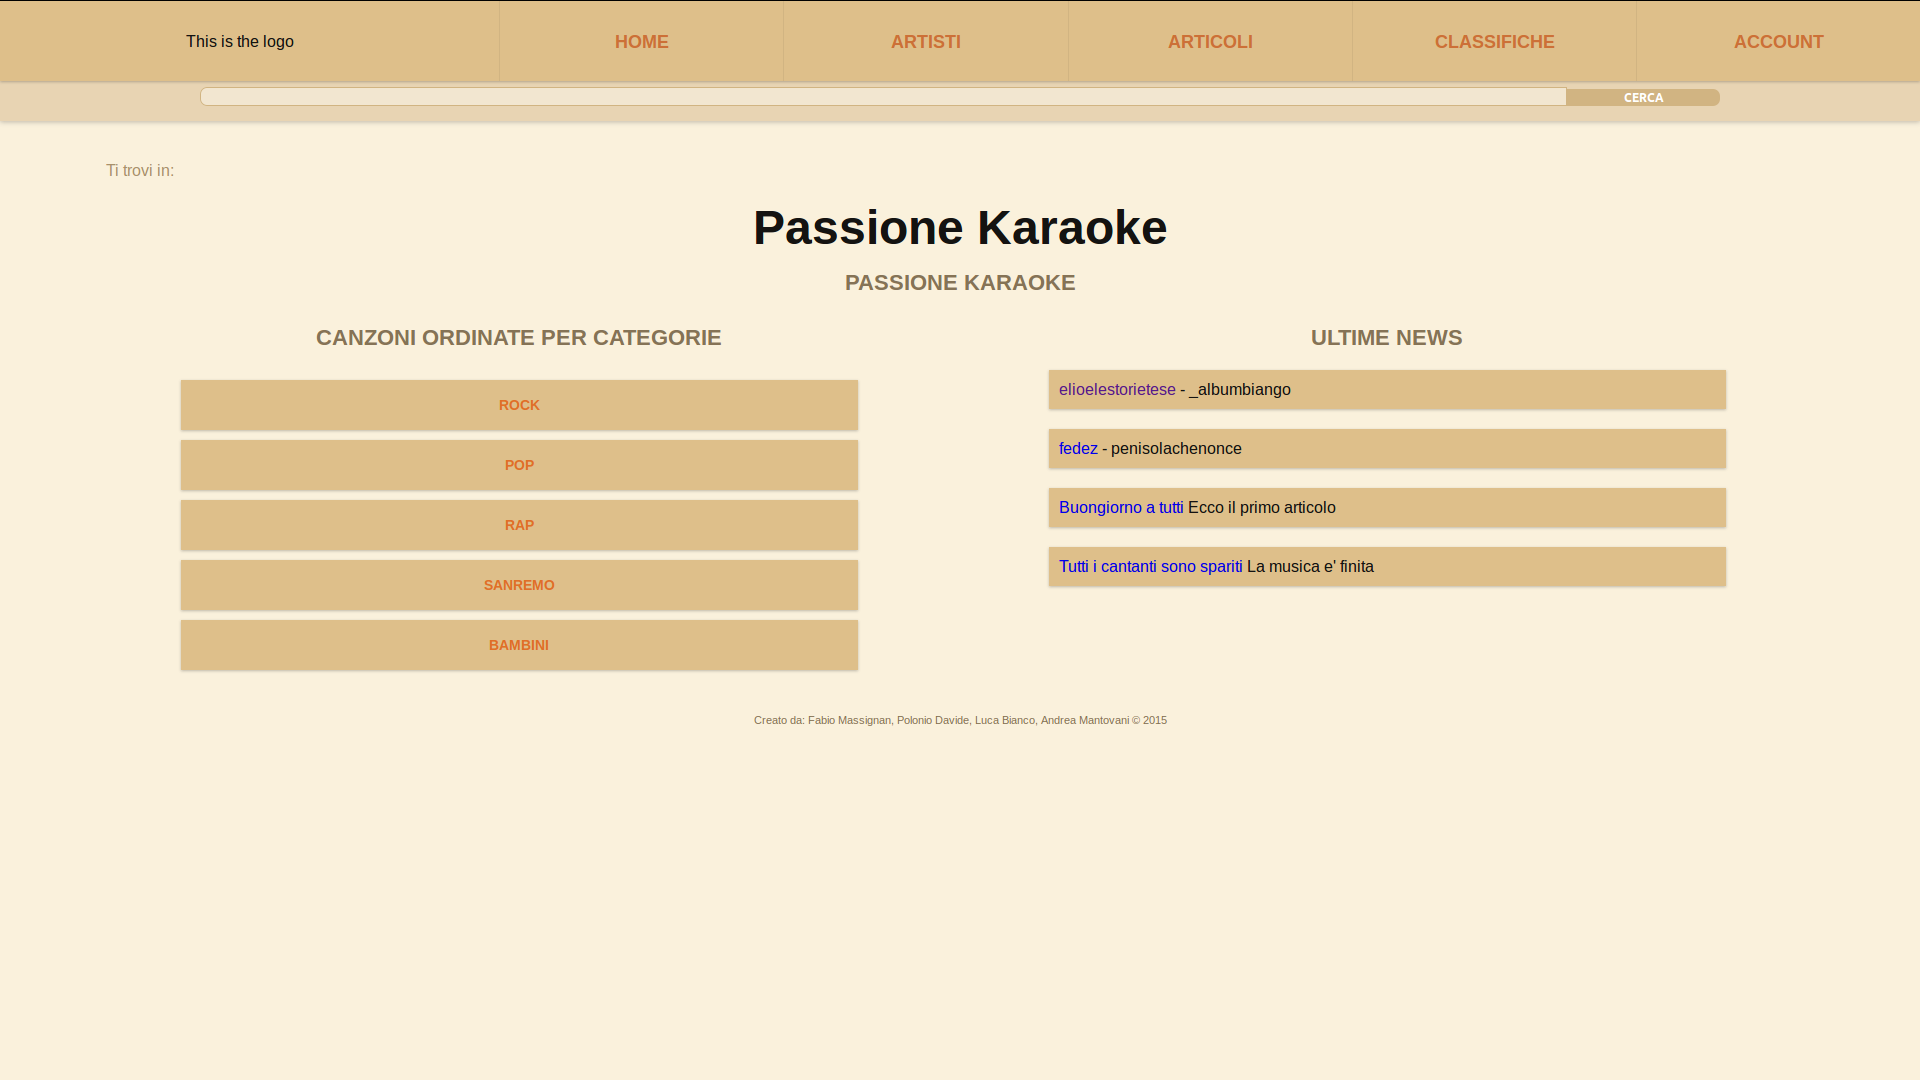
\includegraphics[scale=0.104]{firstImgNormal}
        \caption{Design del sito con vecchi colori}
    \end{subfigure}
    ~
    \begin{subfigure}[b]{0.45\textwidth}
        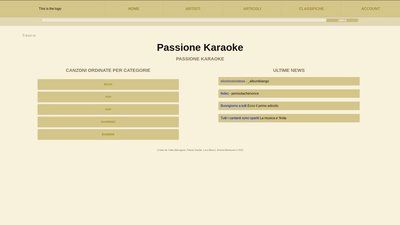
\includegraphics[scale=0.5]{firstImgDeuteranope}
        \caption{Risultati del test per \textit{Deuteranope}}
    \end{subfigure}
    \newline
    \begin{subfigure}[b]{0.45\textwidth}
        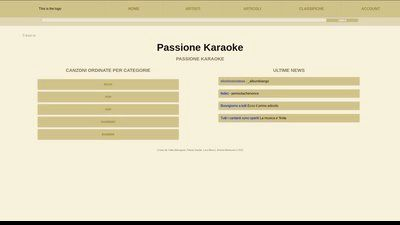
\includegraphics[scale=0.5]{firstImgProtanope}
        \caption{Risultati del test per \textit{Protanope}}
    \end{subfigure}
    ~
    \begin{subfigure}[b]{0.45\textwidth}
        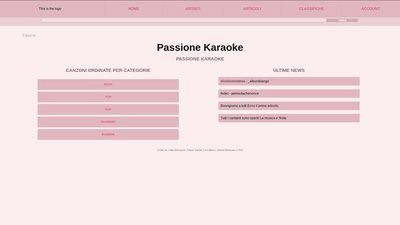
\includegraphics[scale=0.5]{firstImgTritanope}
        \caption{Risultati del test per \textit{Tritanope}}
    \end{subfigure}
    ~
    \caption{Risultato del sito con i colori inizialmente scelti}
\end{figure}


Come si può ben vedere, questa palette di colori non degrada in maniera elegante, e causa invece una distorsione troppo forte. Si è quindi deciso di cambiarli, ottenendo i seguenti risultati:

\begin{figure}[H]
    \centering
    \begin{subfigure}[b]{0.45\textwidth}
        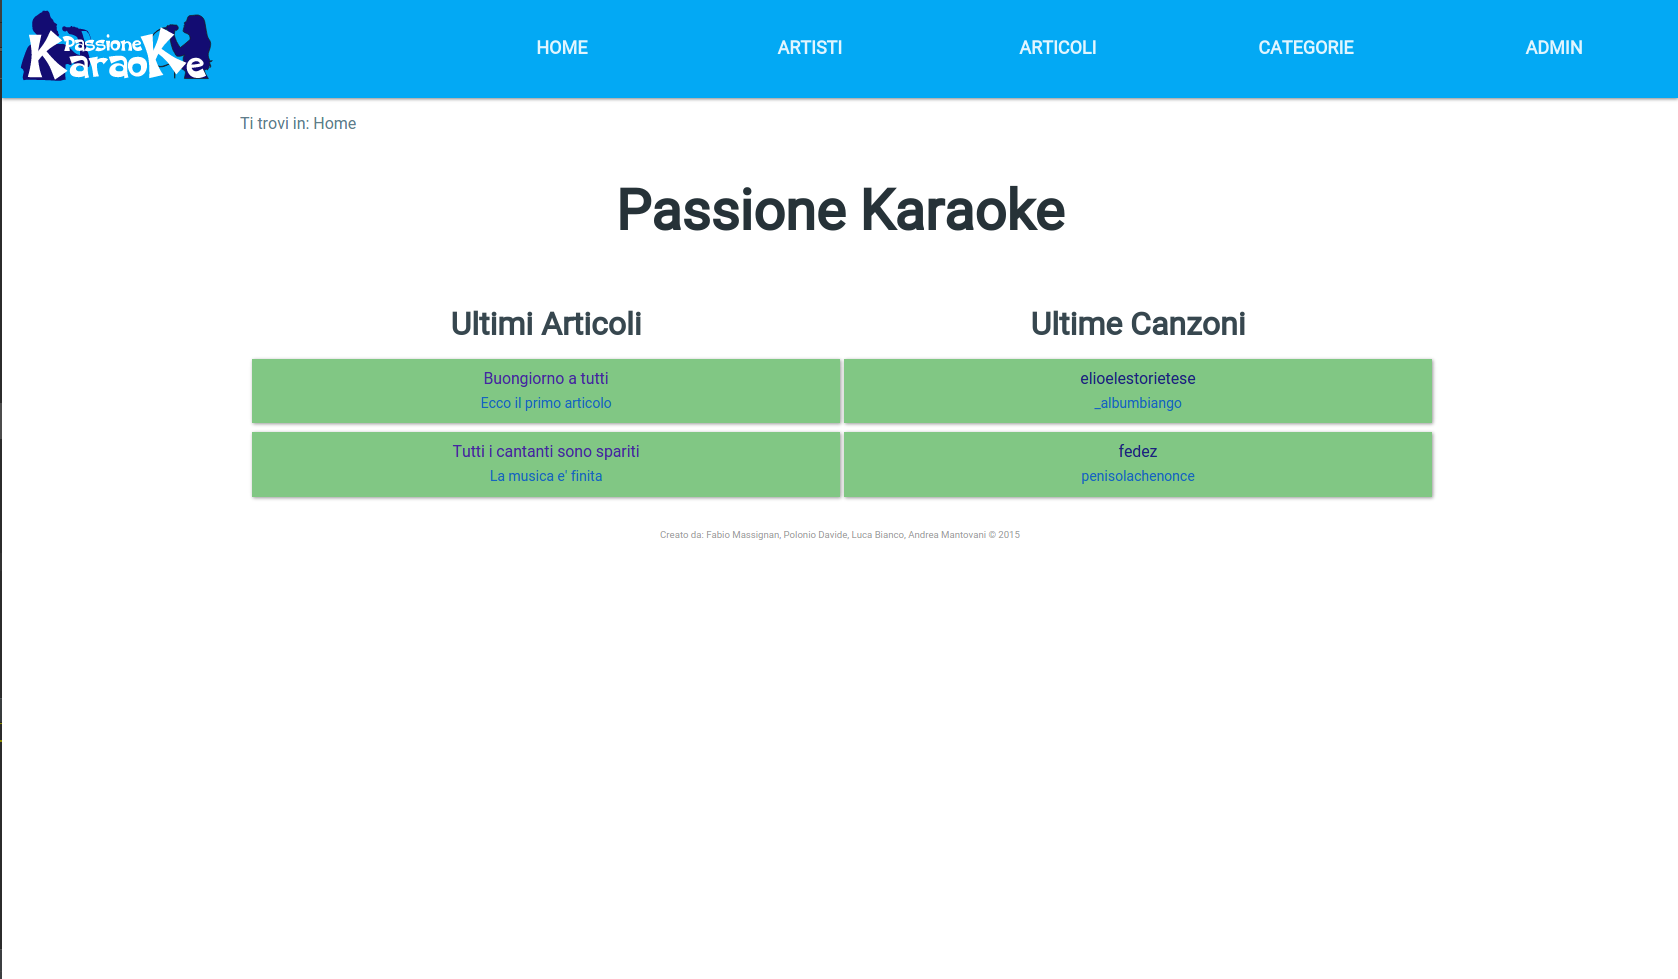
\includegraphics[scale=0.119]{lastImgNormal}
        \caption{Design del sito con i colori finali}
    \end{subfigure}
    ~
    \begin{subfigure}[b]{0.45\textwidth}
        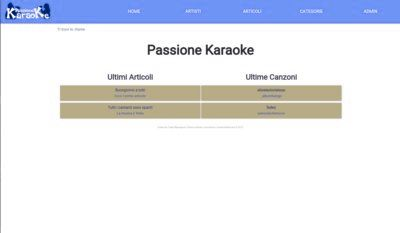
\includegraphics[scale=0.5]{lastImgDeuteranope}
        \caption{Risultati del test per \textit{Deuteranope}}
    \end{subfigure}
    \newline
    \begin{subfigure}[b]{0.45\textwidth}
        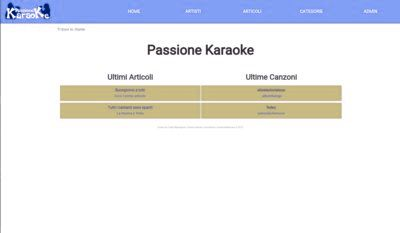
\includegraphics[scale=0.5]{lastImgProtanope}
        \caption{Risultati del test per \textit{Protanope}}
    \end{subfigure}
    ~
    \begin{subfigure}[b]{0.45\textwidth}
        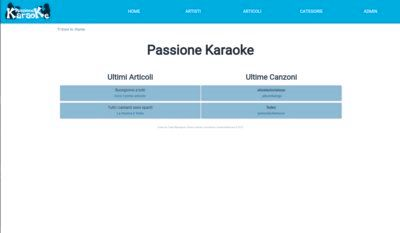
\includegraphics[scale=0.5]{lastImgTritanope}
        \caption{Risultati del test per \textit{Tritanope}}
    \end{subfigure}
    ~
    \caption{Risultato finale dei colori del sito}
\end{figure}


\subsubsection{Colori delle icone per esprimere preferenze}
Per accertarsi di avere un'accessibilit\`a completa dal punto di vista visivo, \`e stato fatto anche il controllo delle icone dei pulsanti per esprimere il giudizio positivo o negativo su una canzone. Questo controllo era necessario in quanto i simboli utilizzati (il microfono rivolto verso l'alto per esprimere un giudizio positivo e il microfono rivolto verso il basso per esprimere un voto negativo) non rappresentano una convenzione standard, ma essendo convenzioni interne del sito, bisognava assicurarsi che tutti gli utenti con percezione dei colori alterata fossero in grado di comprendere a pieno il messaggio trasmesso.

\begin{figure}[H]
    \centering
    \begin{subfigure}[b]{0.4\textwidth}
        
\includegraphics[scale=0.32]{microphoneLike}
        \caption{Icona usata per esprimere un apprezzamento positivo}
    \end{subfigure}
    ~
    \begin{subfigure}[b]{0.4\textwidth}
        
\includegraphics[scale=0.32]{microphoneNotLike}
        \caption{Icona usata per esprimere un apprezzamento negativo}
    \end{subfigure}
    ~
    \caption{Icone usate per esprimere preferenze all'interno del sito}
\end{figure}

\`E importante notare la scelta del blu al posto di un pi\`u comune verde per l'icona per il voto positivo: dopo un test effettuato tramite \url{http://www.vischeck.com/} si \`e notato infatti che l'utilizzo contemporaneo del verde e del rosso non avrebbe reso abbastanza accessibile il riconosciemnto delle icone, in quanto non ci sarebbe stata una distinzione abbastanza forte tra i due colori. Dopo aver cambiato il colore dell'icona di apprezzamento sono stati effettuati nuovamente i test, ottenendo risultati decisamente migliori:
\begin{itemize}

    \item[]

        \begin{figure}[H]
            \centering
            \begin{subfigure}[b]{0.3\textwidth}
                
\includegraphics[scale=0.3]{microphoneLikeDeuteranope}
                \caption{Risultati del test per \textit{Deuteranope}}
            \end{subfigure}
        ~
            \begin{subfigure}[b]{0.3\textwidth}
                
\includegraphics[scale=0.3]{microphoneLikeProtanope}
                \caption{Risultati del test per \textit{Protanope}}
            \end{subfigure}
        ~
            \begin{subfigure}[b]{0.3\textwidth}
                
\includegraphics[scale=0.3]{microphoneLikeTritanope}
                \caption{Risultati del test per \textit{Tritanope}}
            \end{subfigure}
        ~
            \caption{Risultati del test per l'icona per esprimere una preferenza positiva}
        \end{figure}

    \item[]

        \begin{figure}[H]
            \centering
            \begin{subfigure}[b]{0.3\textwidth}
                
\includegraphics[scale=0.3]{microphoneNotLikeDeuteranope}
                \caption{Risultati del test per \textit{Deuteranope}}
            \end{subfigure}
        ~
            \begin{subfigure}[b]{0.3\textwidth}
                
\includegraphics[scale=0.3]{microphoneNotLikeProtanope}
                \caption{Risultati del test per \textit{Protanope}}
            \end{subfigure}
        ~
            \begin{subfigure}[b]{0.3\textwidth}
                
\includegraphics[scale=0.3]{microphoneNotLikeTritanope}
                \caption{Risultati del test per \textit{Tritanope}}
            \end{subfigure}
        ~
            \caption{Risultati del test per l'icona per esprimere una preferenza negativa}
        \end{figure}

\end{itemize}

\newpage

\subsubsection{Contrasto e leggibilit\`a}

\paragraph*{Indice leggibilità}\`E stato dato peso nel progetto anche alla leggibilit\`a del testo per quelle persone che riportano problemi visivi. Per il test sul contrasto tra testo e sfondo si \`e rivelato utile il tool reperibile al seguente indirizzo: \url{http://leaverou.github.io/contrast-ratio/}.
Il valore espresso in scala numerica indica il rapporto cromatico tra lo sfondo e il colore delle scritte. Più alto \`e il valore maggiore è il contrasto.

\paragraph*{Voci menu}I colori delle voci del menu e dello sfondo della barra menu sono stati scelti in maniera tale che avessero un buon contrasto, cercando comunque di mantenere un certo standard di design grafico.
\begin{figure}[H]

    \centering
    
\includegraphics[scale=0.35]{menuContrast}
    \caption{Zoom in dettaglio per evidenziare il contrasto tra i colori delle voci del menu e dello sfondo dello stesso}

\end{figure}

L'indice di contrasto ha dato un valore più che accettabile, come si pu\`o vedere nell'immagine sottostante.
\begin{figure}[H]

    \centering
    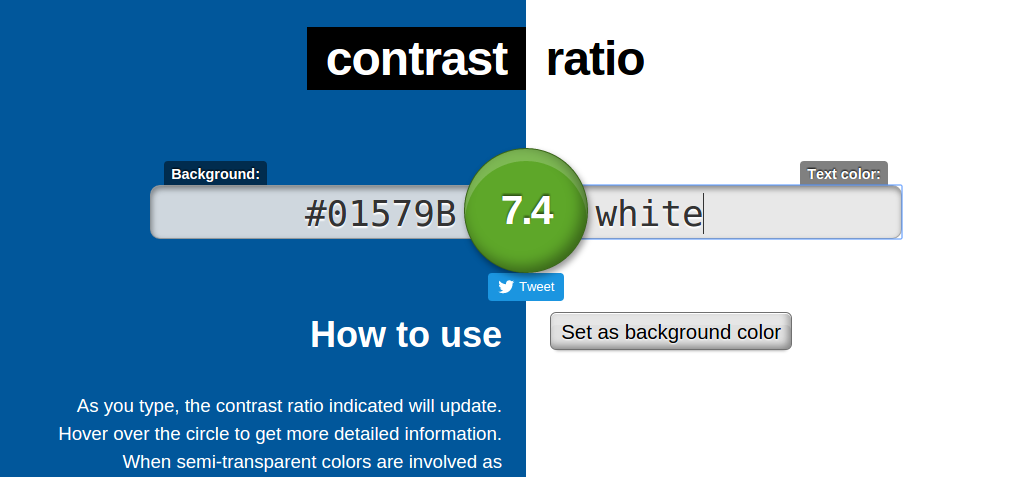
\includegraphics[scale=0.25]{contrastRatioMenu}

\end{figure}


Lo stesso accorgimento è stato adottato anche per il colore delle voci del menu su cui l'utente ha posizionato il mouse. In questo caso \`e stato utile un effetto \textit{hover} tramite CSS, che comunque non ha influenzato la leggibilità.
\begin{figure}[H]

    \centering
    
\includegraphics[scale=0.35]{menuHoverContrast}
    \caption{Zoom in dettaglio del menu in uno stato di \textit{hover}}

\end{figure}

Per il menu in uno stato di \textit{hover} si è ottenuto un valore più basso, che abbiamo ritenuto comunque sufficiente.
\begin{figure}[H]

    \centering
    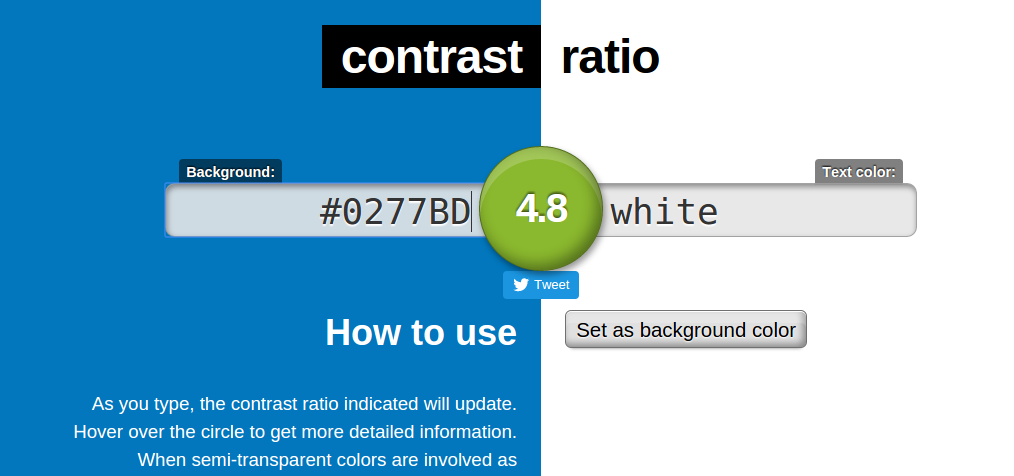
\includegraphics[scale=0.25]{contrastRatioHoverMenu}

\end{figure}


\paragraph*{Lista ultime canzoni/artisti}Il test di leggibilità è stato effettuato anche in questo particolare, per cui è stato deciso di adottare un vivace verde.
\begin{figure}[H]

    \centering
    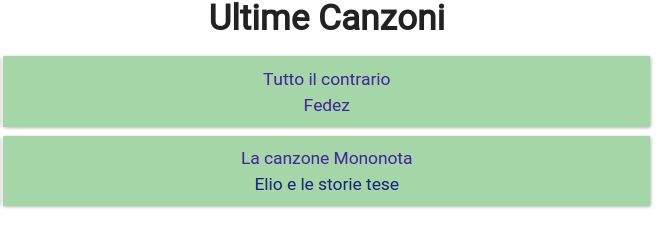
\includegraphics[scale=0.35]{lastSongContrast}
    \caption{Dettaglio del particolare per cui è stato effettuato il test di leggibilità}

\end{figure}

Il test ha ottenuto un punteggio alto, che indica un ottimo rapporto di colori e quindi un'ottima leggibilità da parte di tutti gli utenti del sito.
\begin{figure}[H]

    \centering
    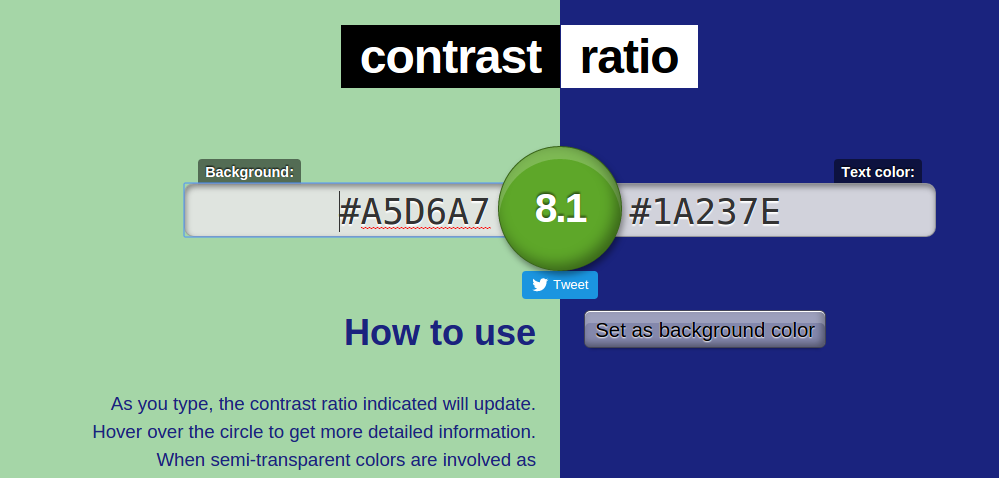
\includegraphics[scale=0.25]{contrastRatioLastSong}

\end{figure}

\paragraph*{Lista di tutti gli artisti}
Per quanto riguarda la sezione contenente la lista di tutti gli artisti, si \`e voluto dare grande attenzione alla leggibilit\`a, in quanto dovrebbe essere la parte pi\`u importante del sito, nonch\`e quella pi\`u visitata dagli utenti.


\begin{figure}[H]

    \centering
    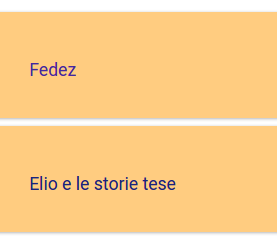
\includegraphics[scale=0.35]{artistsListContrast}
    \caption{Particolare che suggerisce l'alta leggibilità della pagina "Artisti"}

\end{figure}

Il tool con cui sono stati effettuati i test in questo punto ha dato uno dei punteggi più alti in assoluto.
\begin{figure}[H]

    \centering
    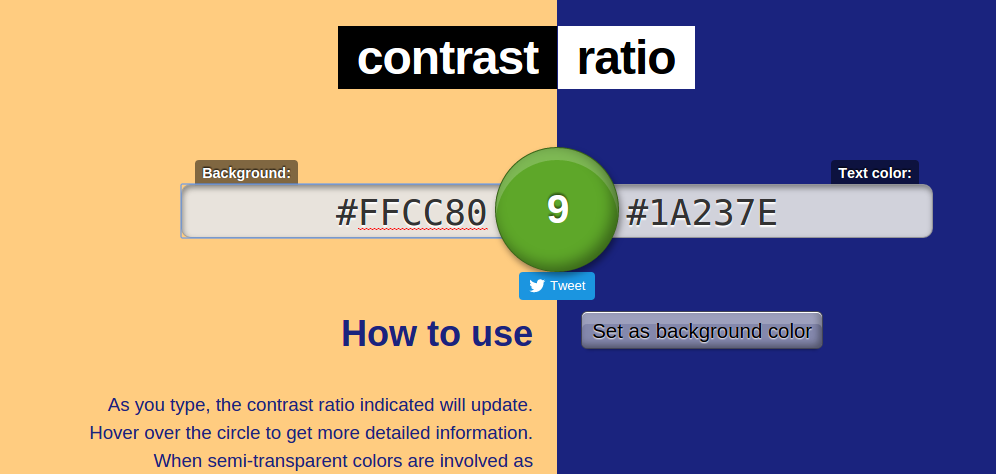
\includegraphics[scale=0.25]{contrastRatioArtistsList}

\end{figure}

\paragraph{Box per gli articoli}È stato analizzato il contrasto anche nel box per gli articoli.
\begin{figure}[H]

    \centering
    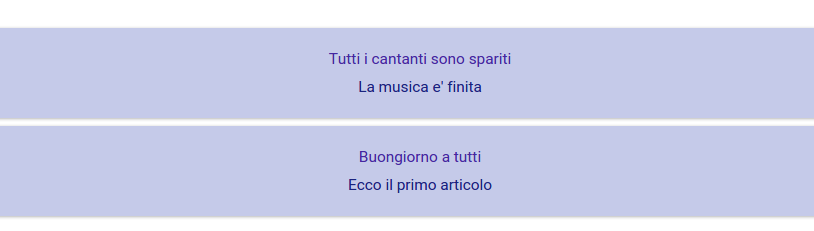
\includegraphics[scale=0.35]{articlesListContrast}

\end{figure}

Il risultato ottenuto è nella media con i precedenti.
\begin{figure}[H]

    \centering
    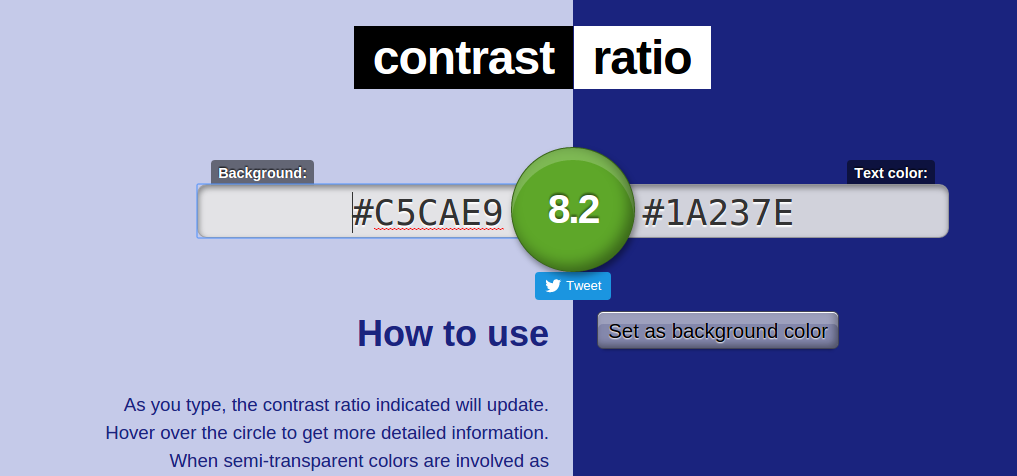
\includegraphics[scale=0.25]{contrastRatioArticleList}

\end{figure}

\paragraph*{Testo generico in articoli e canzoni}Nei contenuti di articoli e canzoni e nel testo generico (come titoli e sottotitoli) si è tenuto un classico contrasto bianco-nero, assicurando il massimo punteggio di leggibilità.

\subsubsection{Form e segnalazione errori}
\label{form-accessibilita}
Durante la navigazione è possibile, da parte dell'utente amministratore, inserire dati tramite l'utilizzo di form (per esempio aggiungere un cantante). È stato quindi necessario rendere i form accessibili tramite diversi accorgimenti:
\begin{itemize}

    \item aggiunta di un bordo per ogni form in modo da rendere chiaro all'utente quali siano i campi form;
    \item nei box di errore specificato in modo chiaro il tipo di errore riscontrato, con un esempio di input corretto. I box vengono posizionati il più vicino possibile al form di input corrispondente.

\end{itemize}
Sono state effettuate anche delle scelte di usabilità, esplicate in \ref{form-usabilita}

\subsubsection{Gestione contenuti}

\paragraph*{Agevolazione per gli utenti usanti screen reader}Per tutti gli utenti che usano gli screen reader, sono stati adottati i seguenti accorgimenti:
\begin{itemize}

    \item inserimento di link all'interno della pagina stessa, nascosti per permettere il salto di contenuti ridondanti nelle pagine (come ad esempio il menu). Il link è stato posto via CSS non visibile agli utenti normali, ma fruibile dagli utenti che utilizzano screen reader;
    \item utilizzo del tag HTML \textit{span}, che ha permesso la corretta pronuncia delle parole in lingua straniera da parte dello screen reader;
    \item presenza di un titolo e di un contenuto alternativo per ogni immagine del sito;

    \item indicazione chiara di ogni contenuto all'interno delle pagine, per aiutare persone con problemi cognitivi;

    \item aggiunta in ogni form di un'etichetta label e raggruppamento dei form in fieldset;

    \item presenza del link a fondo pagina (prima del footer) per dare la possibilità agli screen reader di tornare a inizio pagina;

\end{itemize}
Infine, per dare l'opportunit\`a all'utente che sfrutta una tecnologia sceen reader di visitare il sito in maniera pi\`u lineare, e per aiutare la ricerca di informazioni da parte di quelle persone che hanno disabilit\`a cognitive, \`e stata creata una \textit{Mappa del sito} che fornisce una visione sequenziale di tutti i contenuti, in modo tale da fornire una vista globale del sito. Questo permette all'utente di ottenere quello che desidera senza dover necessariamente passare tra le svariate pagine presenti.

%TODO
